\chapter{Použité technologie}
\label{3-technologie}

Třetí kapitola stručně představuje jednotlivé technologie použité při
tvorbě webového administrátorského rozhraní.

\section{LDAP}
% https://en.wikipedia.org/wiki/Lightweight_Directory_Access_Protocol
% %http://www.openldap.org/doc/admin24/intro.html

Lightweight Directory Access Protocol neboli \zk{LDAP} je otevřený,
standardizovaný protokol pro přístup k adresářovým službám. Slouží k
zobrazování dat, jejich úpravám a ukládání na adresářovém serveru přes
Internet Protocol (\zk{IP}).

Adresářová služba (directory service) je v podstatě specializovaná
databáze, která slouží především k procházení a vyhledávání, ke změnám
dochází jen zřídka. Obvykle neposkytuje komplikovanější databázové
techniky, jako jsou transakce a operace nutné pro zachování datové
integrity. Pro zvýšení rychlosti odezvy mohou dokonce obsahovat i
duplicitní záznamy.

\zk{LDAP} je založen na modelu server-klient. Jeden či více \zk{LDAP}
serverů obsahují data ve stromové struktuře (directory information
tree, DIT). Klient požádá o záznam odpovídající jeho dotazu. Odpověď
dostane buď ze serveru, ke kterému je připojen, nebo je odkázán na
jiný server, kde je informace uložena. Výsledek hledání bude vždy
stejný, ať už se připojí ke kterémukoliv serveru. Tento rys je
důležitý obzvláště u globálních adresářových služeb.

\zk{LDAP} model se skládá z jednotlivých záznamů (entries). Záznam
sestává z kolekce atributů (povinných a nepovinných) a má přiřazen
globálně unikátní identifikátor, tzv. Distinguished Name (\zk{DN}),
který je založen na lokaci záznamu v rámci hierarchického (stromového)
uspořádání modelu. \zk{DN} začíná vlastním jménem záznamu (Relative
Distinguished Name) a k němu jsou jako řetěz připojena jména všech
jeho předků. Každý atribut má vlastní datový typ a může obsahovat
jednu či více hodnot.

Podle uvedené ukázky stromové struktury by jednoznačným pojmenováním
pro uživatele se jménem \textsf{uid=test01} bylo \zk{DN}
\textsf{uid=test01, ou=People, dc=org, dc=com}.

\begin{figure}[H] \centering
      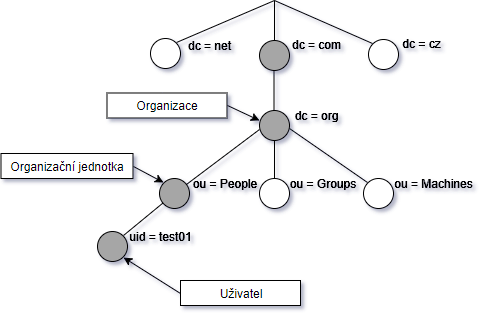
\includegraphics[width=380pt]{./pictures/ldap_dit.png}
      \caption[Příklad stromové struktury LDAP]{Příklad stromové struktury LDAP (zdroj:
	  \href{}{Tereza Kulovaná})}
      \label{fig:ldap-dit}
\end{figure}

\zk{LDAP} poskytuje ochranu informací, které jsou na serveru uloženy,
pomocí mechanismu autentizace, který požaduje po klientovi prokázaní a
ověření identity před zobrazením jakýchkoliv dat.

Server \zk{LDAP} je vhodný pro autentizaci uživatelů a klientských
zařízení, pro správu uživatelských informací, apod. Výhodou je, že
uživatelé potřebují pro přístup k různým aplikacím v síti (pošta, ftp)
pouze jedny přihlašovací údaje. Je nezávislý na operačním systému.

Protokol LDAP vychází ze standardu X.500, jehož je odlehčenou
variantou. Někdy je nazýván
X.500-lite.\footnote{https://www.webopedia.com/TERM/L/LDAP.html}

\newpage
\subsection{OpenLDAP}
\label{openldap}
%http://www.openldap.org/doc/admin24/intro.html

% neznam licenci
\begin{figure}[H] \centering
      
\includegraphics[width=100pt]{./pictures/LDAPlogo.png}
      \caption[OpenLDAP logo]{OpenLDAP logo (zdroj:
	  \href{http://www.openldap.org/images/headers/LDAPlogo.gif}{OpenLDAP.org})}
      \label{fig:ldap}
\end{figure}

OpenLDAP je otevřená (open-source) implementace protokolu \zk{LDAP}
vyvíjená pod hlavičkou OpenLDAP Project. OpenLDAP je distribuován pod
vlastní licencí OpenLDAP Public
License.\footnote{http://www.openldap.org/software/release/license.html}
Vývoj OpenLDAP má počátek v roce 1998 a navazuje na předešlou činnost
University of Michigan.

Hlavní komponenty:
\begin{itemize}
\item slapd - nezávislý \zk{LDAP} server
\item knihovny implementující \zk{LDAP} protokol
\item klientské nástroje (ldapsearch, ldapadd, ldapmodify,...)
\end{itemize}

\textit{slapd} (Standalone \zk{LDAP} daemon) je nezávislý \zk{LDAP}
adresářový server, který zachytává \zk{LDAP}připojení a odpovídá na
operace, které přes tato spojení obdrží. Umožňuje připojení ke
globální \zk{LDAP} adresářové službě nebo může lokální služby
obsluhovat sám. Může běžet na mnoha různých platformách.

Podporuje silnou autentizaci a bezpečnost dat díky metodě SASL (Simple
Authentication and Security Layer) a protokolu TLS (Transport Layer
Security). Poskytuje široké možnosti kontroly přístupu k informacím v
databázi - přístup může být udělen mj. na základě přihlašovacích
údajů, \zk{IP} adresy nebo \zk{DN}. \textit{slapd} nabízí celou škálu
databázových backendů - MDB, hierarchický, vysoce výkonný transakční
databázový backend; SHELL, backend pro shellové skripty; a jednoduchý
backend PASSWD a jiné.

Konfigurace \textit{slapd} probíhá přes konfigurační soubor, příklad takové změny je uveden v kapitole \ref{web-console}. 

%ldapmodify, ldapadd, ldapsearch, ldapdelete?

GIS.lab využívá OpenLDAP 2.4. V rámci webové aplikace probíhá
synchronizace s Djangem, z adresářové struktury OpenLDAP jsou
konkrétně využívány organizační jednotky \textit{People} a
\textit{Groups}. Náhled struktury GIS.labu je v ukázce omezen jen na
záznamy potřebné k vytvoření \zk{DN} těchto organizačních jednotek,
které v realitě obsahují mnohem více záznamů.

\begin{figure}[H] \centering
      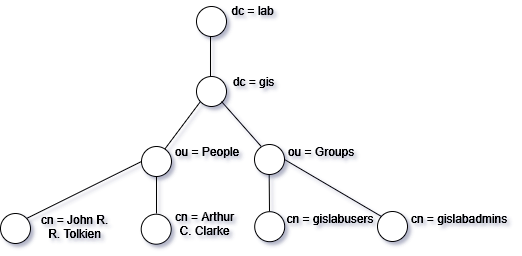
\includegraphics[width=400pt]{./pictures/gislab-ldap_dit.png}
      \caption[Ukázka stromové struktury GIS.labu]{Ukázka stromové struktury GIS.labu (zdroj:
	  \href{}{Tereza Kulovaná})}
      \label{fig:gislab-dit}
\end{figure}

\subsection{django-python3-ldap}
% https://github.com/etianen/django-python3-ldap/blob/master/README.rst
Knihovna \textit{django-python3-ldap} zajišťuje autentizaci uživatelů
s \zk{LDAP} serverem a synchronizaci \zk{LDAP} uživatelů s lokální
databází Djanga. Podporuje vlastní modely Djanga upravené specifickým
potřebám. Ve výchozím nastavení je nakonfigurována podpora přihlášení
přes OpenLDAP, po úpravě nastavení umožňuje připojení k adresářové
službě Microsoft Active Directory. Funguje jak pro Python 2, tak pro
Python 3.

Při prvním přihlášení uživatele se aplikace pokusí vytvořit připojení
k \zk{LDAP} serveru skrze poskytnuté uživatelské jméno a heslo. V
případě úspěšného připojení jsou údaje z \zk{LDAP} serveru uloženy do
databáze Djanga a při každém dalším přihlášení jsou aktualizovány.

Synchronizaci všech uživatelů zároveň zajišťuje příkaz
\textsf{manage.py ldap\_sync\_users}. Tuto akci lze provést
jednorázově, pro pravidelnou synchronizaci může být automatizovaně
spouštěn na pozadí skrze softwarového démona Cron.

Použití této knihovny je relativně snadné. Po instalaci stačí v
konfiguračním souboru Djanga \textit{settings.py} nastavit potřebné
proměnné (např. \zk{URL} adresu \zk{LDAP} serveru) a při příštím
spuštění serveru již synchronizace funguje.

%% ML: tu vetu bych zaclenil nejak do textu, takto pusobi rusive
%% (jeste navic na zacatku stranky)
\textit{django-python3-ldap} vychází z knihovny \textit{ldap3}.

\subsection{ldap3}
%https://ldap3.readthedocs.io/welcome.html
%https://buildmedia.readthedocs.org/media/pdf/ldap3/stable/ldap3.pdf - ldap3 dokumentace
Knihovna \textit{ldap3} je založena na aplikaci protokolu \zk{LDAP}
v3. Poskytuje operace potřebné pro připojení k \zk{LDAP} serveru, pro
vyhledání záznamů, jejich vytvoření, úpravu a odstranění. Podporuje
verze Python 2 i 3.


\section{Python}

\begin{figure}[H] \centering
      
\includegraphics[width=150pt]{./pictures/python-logo-master-v3-TM.png}
      \caption[Python logo]{Python logo (zdroj:
\href{https://www.python.org/static/community_logos/python-logo-master-v3-TM.png}{Python.org})}
      \label{fig:python}
  \end{figure}
  
% (3) https://docs.python.org/3/faq/general.html#general-python-faq

Python je vysokoúrovňový, interpretovaný programovací jazyk. Podporuje
procedurálně i objektově orientované programování, je výkonný, zároveň
má velmi jednoduchou a čistou syntax. V ostatních jazycích je
odsazování řádků doporučeno z hlediska přehlednosti, u Pythonu je
%% ML: odkaz nefunguje
základním stavebním kamenem a je povinné.\cite{Kulovana, 2017}

Dnes je Python vyvíjen jako open source projekt
pod záštitou neziskové organizace Python Software Foundation
(\zk{PSF}). Je distribuován pod licencí \zk{PSF}, která je
kompatibilní s \zk{GPL}. Je možné ho nainstalovat na běžné platformy
jako Windows, Unix nebo Mac OS, pro Linux je většinou součástí
základní instalace. Při vyvarování se systémově závislých funkcí je
přenositelný mezi~platformami bez jakýchkoli změn.

Python má široké využití, od jednoduchých programů po rozsáhlé
aplikace. Právě pro tyto možnosti, univerzálnost, přehlednost kódu a
výkonnost z něj udělaly programovací jazyk, který je mezi začátečníky ve
velké oblibě. Během krátké doby v~něm funkční skript zvládne napsat
každý.

%% ML: jaky ma smysl radek nize?
--

%https://wiki.python.org/moin/Python2orPython3#Which_version_should_I_use.3F
% http://python-notes.curiousefficiency.org/en/latest/python3/questions_and_answers.html#when-can-we-expect-python-2-to-be-a-purely-historical-relic

Python v současnosti existuje ve dvou hlavních verzích - Python 2 a
Python 3. Python 3.0 byl vydán v roce
2008\footnote{https://www.python.org/downloads/} a není zpětně
kompatibilní s verzí Python 2. Hlavním důvodem pro takto zásadní změnu
bylo rozhodnutí Guido van Rossuma, zakladatele jazyku Python, očistit
Python 2.x od mnoha problémů pořádně v jednom kroku.

%% ML: upraveni tradicnich trid (?)
Největšími změnami jsou upravení tradičních tříd a oddělení abstrakcí
\textsf{řetězec} a \textsf{posloupnost bytů}. Textový řetězec
(\textsf{str}) je nově převeden ve výchozím nastavení na typ unicode,
což vytváří konzistentnější a spolehlivější prostředí. Změny doznalo
chování operátoru dělení \textsf{/} celých čísel. Výsledkem je číslo s
plovoucí desetinnou čárkou, na rozdíl od předchozí verze, která
vracela celé číslo (ve verzi 3.x dostupné pod operátorem
\textsf{//}). Mezi nejviditelnější novinky pro běžného uživatele je
přechod od příkazu \textsf{print} k funkci \textsf{print()}.

Python 3 je obecně přívětivější k učení nových uživatelů a je
považován za budoucnost tohoto jazyka. Stále však existuje mnoho
programů, jež fungují na poslední verzi Python 2.7 vydané v roce
2010\footnote{https://www.python.org/downloads/}, která již nedostává
žádné velké aktualizace. Důvody jsou různé - daný projekt byl vyvíjen
v Pythonu 2 a nejsou dostatečné kapacity na jeho přechod na novější
verzi; na některých operačních systémech není Python 3 nainstalovaný a
uživatelé nemají vždy práva si ho sami doinstalovat; existuje potřeba
využívat externí knihovnu, která podporuje pouze Python 2 a není
triviální ji převést do Pythonu 3.

Poslední vydanou stabilní verzí je Python
3.7.\footnote{https://www.python.org, květen 2019}

\section{Django}

\begin{figure}[H] \centering
      
\includegraphics[width=150pt]{./pictures/django-logo-positive.png}
      \caption[Django logo]{Django logo (zdroj:
\href{https://static.djangoproject.com/img/logos/django-logo-positive.png}{Djangoproject.com})}
      \label{fig:django}
  \end{figure}

% http://www.moreware.org/books/The%20Definitive%20Guide%20to%20Django.pdf
% https://docs.djangoproject.com/en/2.2/intro/overview/
% http://www.djangoproject.cz/dokumentace/intro/tutorial01/#intro-tutorial01 - pro české výrazy, ale netřeba uvádět

Django je vysokoúrovňový webový framework napsaný v jazyce Python. Je
%% ML: druha cast vety nenavazuje na prvni
udržované organizací Django Software Foundation (DSF), bezplatné a
vydané pod open-source licencí \zk{BSD}. Název získalo po jazzovém
kytaristovi Djangovi Reinhardtovi.

Hlavním cílem Djanga je usnadnit tvorbu komplexních, databází řízených
webových aplikací. Pro tento účel se řídí zásadou oddělení
zodpovědností (angl. Separation of concerns) a volně navazuje na
architekturu Model-view-controller (\zk{MVC}). Ta sestává ze tří volně
propojených komponent:
\begin{itemize}
\item model (model) - reprezentace dat, k nimž aplikace přistupuje
\item view (pohled) - uživatelské rozhraní
\item controller (řadič) - reakce na žádosti a zajištění změn v pohledu nebo v modelu
\end{itemize}

Poslední vydanou stabilní verzí v době zpracování bylo Django 2.1 a
veškerý další popis uvedený níže platí pro tuto verzi.

Frameworky mají snahu co největší množství práce automatizovat a tak
při vytvoření projektu pomocí příkazu:

\begin{center}
\textsf{django-admin startproject nazev\_projektu}
\end{center}

vznikne automaticky jeho základní kostra, která slouží jako podstata
již fungující Django aplikace.

\dirtree{%
.1 project.			
	.2 mysite.
		.3 \_\_init\_\_.py.
		.3 settings.py.
		.3 urls.py.
		.3 wsgi.py.
	.2 db.sqlite3.
	.2 manage.py.
}

\subsubsection{\_\_init\_\_.py}
Soubor \textit{\_\_init\_\_.py} dává Pythonu najevo, že s adresářem, v
němž se soubor nachází, má být zacházeno jako s balíčkem modulů
Pythonu. Jedná se o prázdný soubor, který se obvykle nijak nemění.

\subsubsection{settings.py}
\label{settings}
Soubor \textit{settings.py} skrývá nastavení Django projektu,
např. jakým způsobem má probíhat autentizace, kde jsou umístěné další
potřebné soubory či informace o použitých databázích a registrovaných
aplikacích.

\subsubsection{urls.py}
\textit{urls.py} obsahuje \zk{URL} cesty pro vytvořený Django projekt,
v podstatě se jedná o jakýsi rejstřík stránky. Implicitně obsahuje
cestu k vestavěné administrátorské konzoli. Při propojení s Django
aplikacemi jsou sem přidány další \zk{URL} adresy.

\subsubsection{wsgi.py}
\zk{WSGI} je specifikace popisující komunikaci mezi webovým serverem a
webovou aplikací nebo frameworkem v jazyce Python. Jedná se o primární
nástroj nasazení programů v Djangu. Soubor \textit{wsgi.py} se v
základu skládá z jednoduché \zk{WSGI} konfigurace, již je možno podle
potřeby dále upravovat.

\subsubsection{manage.py}
% http://www.moreware.org/books/The%20Definitive%20Guide%20to%20Django.pdf
% https://docs.djangoproject.com/en/2.2/topics/migrations/
Nástroj pro příkazový řádek \textit{manage.py} umožňuje spravovat
Django projekt. Tento soubor není po vytvoření nijak upravován.

Pro vývoj aplikace lze použít odlehčený webový server Djanga, na němž
může autor okamžitě začít budovat aplikaci, aniž by byla vyžadována
konfigurace produkčního serveru. Vývojový server provádí kontrolu kódu
a automaticky se po každé uložené změně znovu načte, bez nutnosti
restartu. Tento server se spouští příkazem:

\begin{center}
\textsf{python manage.py runserver 0:8080}
\end{center}

Standardně se vývojový server spouští na interní \zk{IP} adrese a
portu 8000. V~případě, že je třeba zobrazovat webové stránky mimo
stroj, na němž server běží, lze nastavit viditelnost a odlišný port
serveru přidáním parametru \textsf{0:8080}. V takové situaci je
stránka dostupná odkudkoliv při zadání adresy nastavené v proměnné
\textsf{ALLOWED\_HOSTS} v souboru \textit{settings.py} a zvoleného
portu.

Pro práci s databází jsou nezbytné dva základní příkazy:

\begin{center}
\textsf{python manage.py makemigrations}
\end{center}

který vytváří jednotlivé migrační soubory založené na změnách
provedených v~modelech Djanga a

\begin{center}
\textsf{python manage.py migrate}
\end{center}

který tyto změny aplikuje do databáze. V případě, že databáze ještě
neexistuje, tak ji automaticky vytvoří.

Migrace v Djangu funguje podobně jako verzovací systémy -
\textsf{makemigrations} odpovídá příkazu \textsf{commit} a
\textsf{migrate} pak obdobně jako \textsf{push} tyto změny propíše do
databáze.

Poslední z významných funkcí \textit{manage.py} je spouštění
jednotkových testů.

\subsubsection{db.sqlite3}
Výchozí databází v Djangu je relační databáze SQLite. Obsahuje
informace o jednotlivých modelech a vztazích mezi nimi.

% https://docs.djangoproject.com/en/2.2/topics/migrations/#sqlite
SQLite nemá vhodně implementovánu podporu změn, Django ji proto
nahrazuje postupem, kdy vytvoří novou tabulku s novým schématem, data
z původní tabulky překopíruje do nové, starou smaže a novou přejmenuje
podle prvotní. Proto se nedoporučuje tuto databázi používat v
produkci, obzvlášť v případě většího množství dat a častých změn.

Kromě SQLite Django oficiálně podporuje databáze PostgreSQL, MySQL a
Oracle.

\subsection{Webové aplikace}
\label{django-app}
Do projektu lze přidávat webové aplikace, jedna aplikace může být
součástí více projektů. Pro její vytvoření lze užít konzolový nástroj:

\begin{center}
\textsf{python manage.py startapp nazev\_aplikace}
\end{center}

Implicitní struktura aplikace je vždy stejná:

\begin{itemize}
\item \textsf{\_\_init\_\_.py} - určuje aplikaci jako balíček Pythonu
\item \textsf{admin.py} - umožňuje registraci datových modelů
  %% ML: ??
\item \textsf{apps.py} - definuje název aplikace??
\item \textsf{models.py} - umožňuje tvorbu datových modelů
\item \textsf{tests.py} - umožňuje tvorbu jednotkových testů
\item \textsf{views.py} - umožňuje definování pohledových funkcí
\end{itemize}

Každou aplikaci, která má být součástí projektu, je třeba
zaregistrovat v souboru \textit{settings.py} (viz \ref{settings}) v
položce \textsf{INSTALLED\_APPS}.

\section{Docker}
\label{docker}

% kouknout na licenci (můžu používat??)
\begin{figure}[H] \centering
      
\includegraphics[width=150pt]{./pictures/Docker_(container_engine)_logo.png}
      \caption[Docker logo]{Docker logo (zdroj:
\href{https://commons.wikimedia.org/wiki/File:Docker_(container_engine)_logo.png}{Wikimedia Commons})}
      \label{fig:docker}
  \end{figure}
  
% https://docs.docker.com/get-started/
% https://en.wikipedia.org/wiki/Docker_(software)
%% ML: deployment -> cesky pojem
Docker je platforma pro vývoj, deployment a běh aplikací. Poskytuje
jednotné rozhraní pro izolaci procesů do standardizovaných balíčků,
tzv. kontejnerů. Kontej\-nery jsou tvořeny vlastním softwarem,
knihovnami a konfiguračními soubory. Jsou na sobě navzájem nezávislé,
ale mohou mezi sebou komunikovat skrze definované kanály. Na rozdíl od
virtuálních strojů neobsahují kontejnery operační systém, ale sdílejí
%% ML: kernel jadro , mozna + poznamka pod carou, co je jadro OS (viz
%% napr. wikipedia, tu bych se v poznamce pod caru nebal citovat)
kernel s hlavním operačním systémem. Díky tomu je režie při jejich
spuštění výrazně nižší a mají mnohem menší velikost.

Kontejnery jsou vytvořeny z tzv. obrazů (images). Image je spustitelný
balíček, který obsahuje všechno potřebné pro běh aplikace (kód,
knihovny, proměnné prostředí, konfigurační soubory). Využívá se ke
skladování a sdílení aplikací. Z jednoho obrazu je možné spustit
jakékoliv množství kontejnerů.

Docker existuje v placené formě i jako open-source software. Funguje v
prostředí Linuxu, novějších verzích Windows a ve vybraných cloudových
službách. Skládá se ze tří komponent:

\begin{itemize}
\item software - Docker démon, proces, který řídí Docker kontejnery
\item objekty - entity sloužící k sestavení aplikace v Dockeru (např. obrazy, kontejnery, služby)
\item registr - repozitář Docker obrazů
\end{itemize}

\section{Ansible}
\label{ansible}  
% https://docs.ansible.com/ansible/latest/index.html

Ansible je jednoduchý automatizační nástroj, který umožňuje
konfiguraci systémů, víceuzlové nasazení aplikací a orchestraci jiných
pokročilejších úloh. Orchestrace je řízena z jednoho řídícího stroje,
jenž přistupuje ke spravovaným uzlům přes SSH nebo PowerShell. Ansible
využívá architekturu, jež běží bez agentů, tedy na uzly jsou jen
dočasně nainstalovány a spuštěny tzv. moduly pomocí SSH. Ve chvíli,
kdy Ansible uzly neřídí, uzel nespotřebovává žádné prostředky, jelikož
na něm není nainstalován démon, který by sám software spouštěl.

K zápisu znovupoužitelného popisu stavu uzlů jsou vytvářeny Ansible
Playbooks. Jedná se o soubory psané v jazyce YAML, který se vyznačuje
pro člověka snadnou čitelností.
